\documentclass{report}
\usepackage{graphicx}

\usepackage{algorithm}
\usepackage{algorithmicx}
\usepackage{algpseudocode}
\usepackage{amsmath}


\floatname{algorithm}{Algorithm}
\renewcommand{\algorithmicrequire}{\textbf{Input:}}
\renewcommand{\algorithmicensure}{\textbf{Output:}}


\begin{document}

\title{ETERNITY: FUNCTIONS}
\author{Wenshu Li\\Student ID: 40203982}
\date{}
\maketitle

\makeatletter
\let\thetitle\@title
\let\theauthor\@author
\let\thedate\@date
\makeatother





% This will generate a table of contents
\tableofcontents
\newpage
\section{Introduction}
\subsection{Discription}
In mathematics, the gamma function is one commonly used extension of the factorial function to complex numbers, is a meromorphic function defined in the complex range, usually written so that negative integers and 0 are its first order poles.There are various definitions of the gamma function, we selected three of them here:
\begin{itemize}
\item For any positive integer n,
\\$$\Gamma \left ( n\right ) = \left ( n-1 \right )!$$
\item Derived by Daniel Bernoulli, for complex numbers with a positive real part, the gamma function is defined via a convergent improper integral:
\\$$\Gamma \left ( n\right ) = \int_{0}^{+\infty} x^{z-1} e^{-x}\mathrm{d}x,  \Re\left ( z \right )>0$$
\item The gamma function on real number field is defined as:
\\$$\Gamma \left ( x \right ) =\int_{0}^{+\infty } t^{x-1} e^{-t} \mathrm{d}t \left (  x>0\right ) $$
\end{itemize} 

\begin{figure}[h]
\caption{Gamma function}
\centering
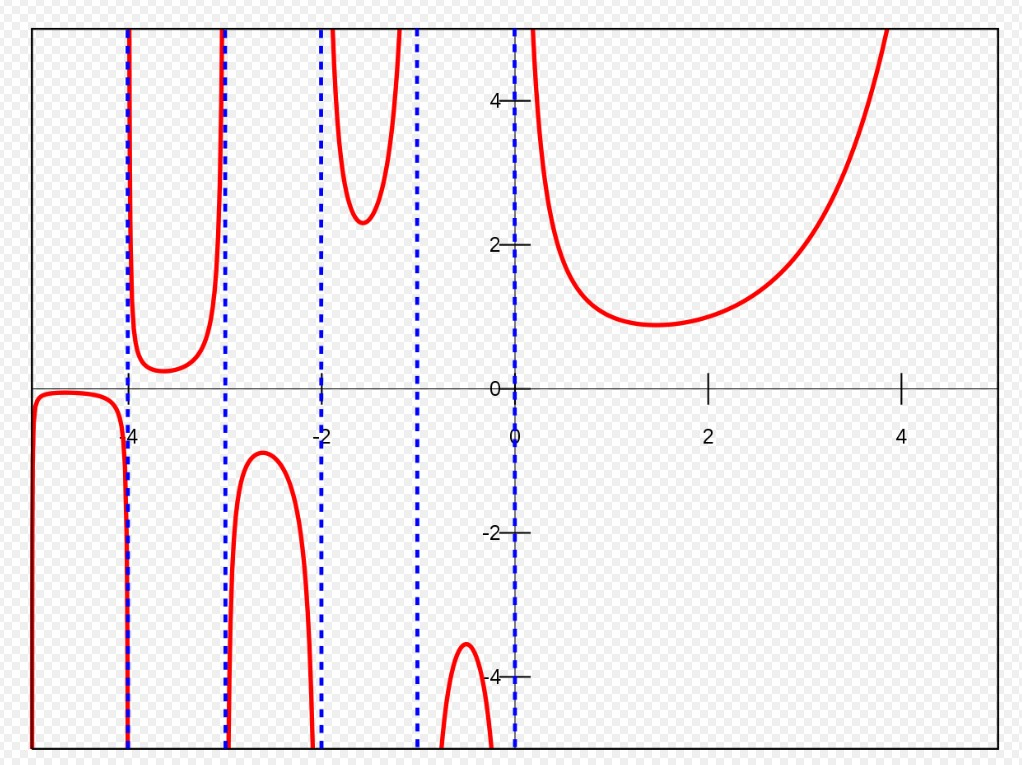
\includegraphics[width=0.5\textwidth]{gamma}
\end{figure}
\subsection{Stakeholders}
\begin{itemize}
\item User1: Mathematicians and researchers in the fields of calculus, mathematical analysis, statistics.
\item User2: Algorithm designers, researchers,engineers in the field of scientific computing in computer and software engineering.
\item User3: People with low maths and programming background who need to obtain the values of gamma function. 
\end{itemize}
\subsection{Domain}
All complex numbers except those whose real part are non-positive integers.
\\$$C/\{n\in Z, n\le 0\}$$
\subsection{Co-Domain}
All real numbers excluding zero.
\\$$\left ( -\infty,0  \right )\cup \left ( 0,+\infty  \right )$$
\subsection{Properties}
%https://en.wikipedia.org/wiki/Gamma_function#Properties
One of the important functional equatuations for the gamma fucntion is Euler's reflection formula:
\\$$\Gamma \left ( 1-z \right ) \Gamma \left ( z \right ) =\frac{\pi }{\sin \pi z},  z \notin Z $$ 
\\which implies,
\subsection{Perticular Values}
%https://en.wikipedia.org/wiki/Gamma_function#Particular_values
Including up to the first 20 digits after the decimal point, some of particular values of the gamma function are:
\begin{itemize}
\item $\Gamma \left ( -\frac{3}{2}  \right ) =\frac{4\sqrt{\pi } }{3} \approx +2.36327180120735470306$
\item $\Gamma \left ( -\frac{1}{2}  \right ) =-2\sqrt{\pi }  \approx -3.54490770181103205459$
\item $\Gamma \left ( \frac{1}{2}  \right ) =\sqrt{\pi }  \approx +1.77245385090551602729$
\item $\Gamma \left ( 1  \right ) =0! = +1$
\item $\Gamma \left ( \frac{3}{2}  \right ) =\frac{\pi }{2}   \approx +0.88622692545275801364$
\item $\Gamma \left ( 2 \right ) =1!=+1$
\item $\Gamma \left ( \frac{5}{2}  \right ) =\frac{3\sqrt{\pi } }{4} \approx +1.32934038817913702047$
\item $\Gamma \left ( 3  \right ) =2! \approx +2$
\item $\Gamma \left ( \frac{7}{2}   \right ) =\frac{15\sqrt{\pi } }{8}  \approx +3.32335097044784255118$
\item $\Gamma \left ( 4 \right ) =3!=+6$
\end{itemize}
\section{Requirements}
\subsection{Functional Requirements}
\begin{itemize}
\item FR1: We shall only consider the positive value as input value.
\item FR2: We shall only consider the real number as input value, ignore the imaginary part.
\item FR3: When the function value exceeds the maximum the value of a double type variable, the function will return NaN.
\end{itemize}
\subsection{Assumptions}

\section{Algorithm}
\subsection{Integrals Method}
\subsubsection{Description}
The first algorithm is based on the Gamma function formula derived by Daniel Bernoulli, using an approximating integrals method called trapezoidal rule. It is used for initial value problems. In calculus, the trapezoidal rule is a technique for approximation the definite integral. This algorithm involves two sub-functions. One is the power function, which given base and exponent as double type arguments, returns $base^{exponent}$. And the exp function, which given exponent as double type argument, returns $e^{exponent}$ .

\subsection{Lanczos Approximation}
\subsubsection{Description}
The second algorithm is based on Lanczos approximation. In mathematics, the Lanczos approximation is a method for computing the gamma function numerically, published by Cornelius Lanczos in 1964. It is a practical alternative to the more popular Stirling's approximation for calculating the gamma function with fixed precision. This algorithm also involves power function, exp function, and sqrt function which given one double type argument, returns square root.
\clearpage
\subsection{Pseudocode} 
\begin{algorithm}
	\caption{Calculate Gamma function using integrals method} 
	\begin{algorithmic}[1]
	\begin{footnotesize}
		\Require Input value of x
		\Ensure Output value of Gamma function
		\Function{$f_y$}{$x$}
			\State \Return {$s^{x-1}*e^{-s}$}
		\EndFunction
		\State
		\Function{$gamma$}{$x$}
			\State $output \gets Error$
			\If{$x<0$}
				\State $result \gets Negative \ input \ is \ not \ allowed.$
			\ElsIf{$x>170$}
				\State $result \gets Infinity$
			\Else
			\State $result \gets 0, intervalGap \gets 10^{-3},i \gets 0$
			\While{$i<a \ particular \ value$}
				\State $result \gets result + \frac{1}{2}*intervalGap*\left ( f_y\left ( i \right ) +y\left (  i-intervalGap\right )  \right )$
				\State $i \gets i+intervalGap$
			\EndWhile
			\State $output \gets result$
			\EndIf
			\State \Return {$output$}
		\EndFunction
	\end{footnotesize}
	\end{algorithmic}
\end{algorithm}
\begin{algorithm} 
	\caption{Calculate Gamma function using Lanczos approximation} 
	\begin{algorithmic}[1]
	\begin{footnotesize}
		\Require Array p as a coefficients, and a constant EPSILON
		\Ensure Output value of Gamma function
		\Function{$gamma$}{$x$}
		\If{$x<0$}
			\State \Return {$Negative \ input \ is \ not \ allowed.$}
		\EndIf
		\If{$x<0.5$}
			\State \Return {$ \frac{\pi}{\sin \left ( \pi*z  \right )*gamma\left ( 1-z \right ) } $}
		\Else
			\State $x \gets x-1$
			\State $z \gets 0.99999999999980993$
			\For{$\left (i,pval\right) in \ p$}
				\State $ z \gets z+\frac{pval}{x+i+1} $
			\EndFor
			\State $t \gets x+length \left (p \right)-0.5$
			\State $m \gets \sqrt{2*\pi }*pow\left ( t,\left ( x+0.5 \right )  \right ) *exp\left ( -t \right ) *z$
		\EndIf
		\State \Return $m$
		\EndFunction
	\end{footnotesize}
	\end{algorithmic}
\end{algorithm}
\clearpage
\subsection{Advantages and Disadvantages}
\subsubsection{Algorithm 1}
Advantages:
\begin{enumerate}
\item Using the the integral method makes the algorithm more intuitive and easy to understand.
\item More precise calculations results can be obtained.
\item The entire algorithm involves loops without recurtion, it requires less memory from computing devices.
\end{enumerate}
Disadvantages:
\begin{enumerate}
\item When the input value is large, it takes significantly longer to produce the result.
\end{enumerate}

\subsubsection{Algorithm 2}
Advantages:
\begin{enumerate}
\item The algorithm makes computing the gamma function becomes a matter of evaluating only a small number of elementary functons and multiplying by stored constants.Simpler to implement.
\item Calculation time is almost independent of the input value.
\end{enumerate}
Disadvantages:
\begin{enumerate}
\item Less precise calculations results than Algorithm 1.
\item The coefficients and Constants that we give in advance are not always precise and accurate.
\end{enumerate}
\subsection{Final Decision}
The algorithm 1 is chosen for implementation. Because it could provide more precise results, although it is theoretically slower than the second one, there is no much difference in terms of actual execution time.
\section{References}
But I don't want my section to be numbered. 
function = $\Gamma$
$\sqrt{1-\frac{v^2}{c^2}}$
\#\LaTeX\textbf{Rules}\!
\begin{itemize}
\item Item 1.
\item Item 2.
\item \ldots
\item Item n.
\end{itemize}
\begin{enumerate}
\item Item 1.
\item Item 2.
\item Item 3.
\end{enumerate}
\end{document}
